\subsection{Combining instance models}
\label{subsec:transformation_framework:instance_models_and_instance_graphs:combining_instance_models}

The structure of \cref{fig:transformation_framework:instance_models_and_instance_graphs:structure_instance_models_graphs} shows that the instance models $Im_A$ and $Im_B$ are combined into one instance model $Im_{AB}$. This section provides the definition of this combination and its corresponding theorems. Please note that the definitions presented here are as generic as possible, and do not actively take into account that $Im_{A}$ and $Im_{B}$ are mostly distinct. This bit of information is added later as part of a theorem and proof.

\begin{defin}[Combination function on type models]
\label{defin:transformation_framework:instance_models_and_instance_graphs:combining_instance_models:combine}
$\mathrm{combine}$ is a binary function on two instance models which combines two instance models into one instance model. Assume $Im_A$ is an instance model typed by type model $Tm_A$ and $Im_B$ is an instance model typed by type model $Tm_B$, then $\mathrm{combine}(Im_A, Im_B)$ is typed by $\mathrm{combine}(Tm_A, Tm_B)$ and is defined as follows:
\begin{align*}
\mathrm{combine}(Im_A, Im_B) = \langle&
Object = Object_{Im_A} \cup Object_{Im_B} \\&
\mathrm{ObjectClass} = \mathrm{objectclass\_\!combine}(Im_A, Im_B) \\&
\mathrm{ObjectId} = \mathrm{objectid\_\!combine}(Im_A, Im_B) \\&
\mathrm{FieldValue} = \mathrm{fieldvalue\_\!combine}(Im_A, Im_B) \\&
\mathrm{DefaultValue} = \mathrm{defaultvalue\_\!combine}(Im_A, Im_B)\rangle
\end{align*}

In which $\mathrm{objectclass\_\!combine}$ is given as part of \cref{defin:transformation_framework:instance_models_and_instance_graphs:combining_instance_models:objectclass_combine}, $\mathrm{objectid\_\!combine}$ as part of \cref{defin:transformation_framework:instance_models_and_instance_graphs:combining_instance_models:objectid_combine}, $\mathrm{fieldvalue\_\!combine}$ as part of \cref{defin:transformation_framework:instance_models_and_instance_graphs:combining_instance_models:fieldvalue_combine} and $\mathrm{defaultvalue\_\!combine}$ as part of \cref{defin:transformation_framework:instance_models_and_instance_graphs:combining_instance_models:defaultvalue_combine}.
\isabellelref{imod_combine}{Ecore.Instance_Model_Combination}
\end{defin}

The combination of two instance models knows a surprisingly simple definition. This is mostly caused by the fact that an instance model only contains of a set of objects, which has some properties. The properties of each object are specified by the different functions, which will be introduced in the following definitions.

First, the function for the combination of object classes is discussed.

\begin{defin}[Combination function for object classes]
\label{defin:transformation_framework:instance_models_and_instance_graphs:combining_instance_models:objectclass_combine}
$\mathrm{objectclass\_\!combine}$ is a partial function on two instance models which returns a new function \\$Object_{Im_{AB}} \Rightarrow Class_{Tm_{AB}}$. It is defined as follows:
\begin{multline*}
    \mathrm{objectclass\_\!combine}(Im_{A}, Im_{B}, o) = \\
        \begin{cases}
        \mathrm{ObjectClass}_{Im_A}(o) & \mathrm{if }\ o \in Object_{Im_A} \cap Object_{Im_B} \land \mathrm{ObjectClass}_{Im_A}(o) = \mathrm{ObjectClass}_{Im_B}(o) \\
        \mathrm{ObjectClass}_{Im_A}(o) & \mathrm{if }\ o \in Object_{Im_A} \setminus Object_{Im_B} \\
        \mathrm{ObjectClass}_{Im_B}(o) & \mathrm{if }\ o \in Object_{Im_B} \setminus Object_{Im_A}
    \end{cases}
\end{multline*}
\isabellelref{imod_combine_object_class}{Ecore.Instance_Model_Combination}
\end{defin}

The combination of two instance models knows a surprisingly simple definition. Because an instance model is essentially a set of objects with properties, no complex definition is needed. The properties of each object are specified by the different functions, which will be introduced in the following definitions.

First, the function of the combination of object classes is discussed.

\begin{defin}[Combination function for object identifiers]
\label{defin:transformation_framework:instance_models_and_instance_graphs:combining_instance_models:objectid_combine}
$\mathrm{objectid\_\!combine}$ is a partial function on two instance models which returns a new function \\$Object_{Im_{AB}} \Rightarrow Name$. It is defined as follows:
\begin{multline*}
    \mathrm{objectid\_\!combine}(Im_{A}, Im_{B}, o) = \\
        \begin{cases}
        \mathrm{ObjectId}_{Im_A}(o) & \mathrm{if }\ o \in Object_{Im_A} \cap Object_{Im_B} \land \mathrm{ObjectId}_{Im_A}(o) = \mathrm{ObjectId}_{Im_B}(o) \\
        \mathrm{ObjectId}_{Im_A}(o) & \mathrm{if }\ o \in Object_{Im_A} \setminus Object_{Im_B} \\
        \mathrm{ObjectId}_{Im_B}(o) & \mathrm{if }\ o \in Object_{Im_B} \setminus Object_{Im_A}
    \end{cases}
\end{multline*}
\isabellelref{imod_combine_object_id}{Ecore.Instance_Model_Combination}
\end{defin}

As mentioned before, the definition of the combination function of object identifiers is very similar to the definition of the combination function of object classes. If an object only occurs in one of the instance models, its identifier is copied over. If an object appears in both instance models, they must have the same identifier already in order to have an identifier in the final model.

A careful reader might notice that the behaviour of the function is strange. Theoretically, it might give rise to double identities, which is undesired. As will be shown later, the combination function and theorems assume that the identities of the models are already distinct. This assumption is fair, as it is possible to redefine two instance models to have distinct identities, without loss of significance.

The following definition describes the combination of field values.

\begin{defin}[Combination function for field values]
\label{defin:transformation_framework:instance_models_and_instance_graphs:combining_instance_models:fieldvalue_combine}
$\mathrm{fieldvalue\_\!combine}$ is a partial function on two instance models which returns a new function \\$(Object_{Im_{AB}} \times Field_{Tm_{AB}}) \Rightarrow Value_{Im_{AB}}$. It is defined as follows:
\begin{multline*}
    \mathrm{fieldvalue\_\!combine}(Im_A, Im_B, ( o, f )) = \\
    \begin{cases}
        \mathrm{FieldValue}_{Im_A}(( o, f )) & \mathrm{if}\ o \in Object_{Im_A} \cap Object_{Im_B}\ \land\\&\quad f \in \mathrm{fields}_{Tm_A}(\mathrm{ObjectClass}_{Im_A}(o))\ \land\\&\quad f \in \mathrm{fields}_{Tm_B}(\mathrm{ObjectClass}_{Im_B}(o))\ \land\\&\quad \mathrm{FieldValue}_{Im_A}(( o, f )) = \mathrm{FieldValue}_{Im_B}(( o, f )) \\
        \mathrm{FieldValue}_{Im_A}(( o, f )) & \mathrm{if}\ o \in Object_{Im_A} \land f \in \mathrm{fields}_{Tm_A}(\mathrm{ObjectClass}_{Im_A}(o))\ \land\\&\quad (o \not\in Object_{Im_B} \lor f \not\in \mathrm{fields}_{Tm_B}(\mathrm{ObjectClass}_{Im_B}(o))) \\
        \mathrm{FieldValue}_{Im_B}(( o, f )) & \mathrm{if}\ o \in Object_{Im_B} \land f \in \mathrm{fields}_{Tm_B}(\mathrm{ObjectClass}_{Im_B}(o))\ \land\\&\quad (o \not\in Object_{Im_A} \lor f \not\in \mathrm{fields}_{Tm_A}(\mathrm{ObjectClass}_{Im_A}(o)))
    \end{cases}
\end{multline*}
\isabellelref{imod_combine_field_value}{Ecore.Instance_Model_Combination}
\end{defin}

The definition of the combination function of field values is a lot more complicated than the previous ones. The function domain causes this complexity. Not every combination of an object and a field has a value. An object only has values for those fields that are defined for its class or superclasses.

When a value is set on one of the instance models, but not the other, the value is copied. Furthermore, if a combination of object and field is set for both instance models and the value is the same, it is also copied. Please note that equality is used here, instead of equivalence. This property is to support some mathematical properties later on. Since the transformation framework will not allow for shared fields anyhow, this will not impose problems later.

The last function that needs to be defined is the combination function for default values. It is given in the following definition.

\begin{defin}[Combination function for default values]
\label{defin:transformation_framework:instance_models_and_instance_graphs:combining_instance_models:defaultvalue_combine}
$\mathrm{defaultvalue\_\!combine}$ is a partial function on two instance models which returns a new function \\$Constant_{Tm_{AB}} \Rightarrow Value_{Im_{AB}}$. It is defined as follows:
\begin{multline*}
    \mathrm{defaultvalue\_\!combine}(Im_{A}, Im_{B}, c) = \\
    \begin{cases}
        \mathrm{DefaultValue}_{Im_A}(c) & \mathrm{if }\ c \in Constant_{Tm_A} \cap Constant_{Tm_B}\ \land\\&\quad \mathrm{DefaultValue}_{Im_A}(c) = \mathrm{DefaultValue}_{Im_B}(c) \\
        \mathrm{DefaultValue}_{Im_A}(c) & \mathrm{if }\ c \in Constant_{Tm_A} \setminus Constant_{Tm_B} \\
        \mathrm{DefaultValue}_{Im_B}(c) & \mathrm{if }\ c \in Constant_{Tm_B} \setminus Constant_{Tm_A}
    \end{cases}
\end{multline*}
\isabellelref{imod_combine_default_value}{Ecore.Instance_Model_Combination}
\end{defin}

The definition of the combination function of default values is very similar to the combination function of constant types of type models (see \cref{defin:transformation_framework:type_models_and_type_graphs:combining_type_models:consttype_combine}). This function gives values to constants defined on the type model level. When a constant only appears in the type model of one of the instance models, the value can be copied from that instance model. This behaviour is logical since the other instance model cannot have a value set for that constant. If a constant is set for both of the corresponding type models, the value set on the instance models must be the same. If this is the case, the value can be copied over. This behaviour is desired, as the value for a constant should not change after the combination of two instance models.

Like the last definition, equality is used here to compare the values, instead of equivalence. Once more, this has been done to support some mathematical properties later on. Since the transformation framework will not allow for shared constants anyhow, this will not impose problems later.

With all definitions in place, it is possible to provide an example. Let us return to the multi-protocol chat application example introduced in \cref{fig:transformation_framework:type_models_and_type_graphs:combining_type_models:combine_example} of \cref{subsec:transformation_framework:type_models_and_type_graphs:combining_type_models}. An instance model for $Tm_{Chat}$ (\cref{fig:transformation_framework:type_models_and_type_graphs:combining_type_models:combine_example_tmod1}) could have an instance of a $\type{Thread}$ with some $\type{Message}$s. Formally, the instance model could look as follows:

\begin{align*}
Im_{Chat} =\ &\langle&
Object =\ &\{ 1, 2, 3 \} \\&&
\mathrm{ObjectClass} =\ &\{
( 1, \type{.Thread} ),
( 2, \type{.Message} ),
( 3, \type{.Message} )
\} \\&&
\mathrm{ObjectId} =\ &\{
( 1, \text{Thread42} ),
( 2, \text{Message4084} ),
( 3, \text{Message4093} )
\} \\&&
\mathrm{FieldValue} =\ &\Big\{
\Big( \big( 1, ( \type{.Thread}, \type{id} ) \big), \big[ \type{string}, \text{``BLUB-E\_Thread\_01''} \big] \Big),\\&&&
\Big( \big( 1, ( \type{.Thread}, \type{proto} ) \big), \big[ \type{enum}, ( \type{.Protocol}, \type{BLUB\!-\!E} ) \big] \Big),\\&&&
\Big( \big( 1, ( \type{.Thread}, \type{messages} ) \big), \big[ \type{seqof}, \big\langle [ \type{obj}, 2 ], [ \type{obj}, 3 ] \big\rangle \big] \Big),\\&&&
\Big( \big( 2, ( \type{.Message}, \type{text} ) \big), \big[ \type{string}, \text{``This is a test''} \big] \Big),\\&&&
\Big( \big( 3, ( \type{.Message}, \type{text} ) \big), \big[ \type{string}, \text{``Did you receive it?''} \big] \Big)
\Big\} \\&&
\mathrm{DefaultValue} =\ &\{\}
\\&\rangle
\end{align*}

A visual representation of this instance model is included in \cref{fig:transformation_framework:instance_models_and_instance_graphs:combining_instance_models:combine_example_imod1}. Now, assume that there also exists some instance model that is typed by the extension represented by $Tm_{Extension}$. This instance model introduces a $\type{Contact}$ instance for the $\type{Thread}$ instance in $Im_{Chat}$. Formally, this instance model could be defined as follows:

\begin{align*}
Im_{Extension} =\ &\langle&
Object =\ &\{ 1, 4 \} \\&&
\mathrm{ObjectClass} =\ &\{
( 1, \type{.Thread} ),
( 4, \type{.Contact} )
\} \\&&
\mathrm{ObjectId} =\ &\{
( 1, \text{Thread42} ),
( 4, \text{Broodkast} )
\} \\&&
\mathrm{FieldValue} =\ &\Big\{
\Big( \big( 1, ( \type{.Thread}, \type{contact} ) \big), \big[ \type{obj}, 4 \big] \Big),\\&&&
\Big( \big( 4, ( \type{.Contact}, \type{id} ) \big), \big[ \type{data}, \text{``BLUB-E\_PubKey\_a8138''} \big] \Big),\\&&&
\Big( \big( 4, ( \type{.Contact}, \type{name} ) \big), \big[ \type{string}, \text{``Lukas''} \big] \Big)
\Big\} \\&&
\mathrm{DefaultValue} =\ &\{\}
\\&\rangle
\end{align*}

The visual representation of $Im_{Extension}$ is included in \cref{fig:transformation_framework:instance_models_and_instance_graphs:combining_instance_models:combine_example_imod2}. With these instance models formally defined, it is possible to combine them using \cref{defin:transformation_framework:instance_models_and_instance_graphs:combining_instance_models:combine}. This will yield the following model:

\begin{align*}
Im_{ChatExt} =\ &\langle&
Object =\ &\{ 1, 2, 3, 4 \} \\&&
\mathrm{ObjectClass} =\ &\{
( 1, \type{.Thread} ),
( 2, \type{.Message} ),
( 3, \type{.Message} ),
( 4, \type{.Contact} )
\} \\&&
\mathrm{ObjectId} =\ &\{
( 1, \text{Thread42} ),
( 2, \text{Message4084} ),
( 3, \text{Message4093} ),
( 4, \text{Broodkast} )
\} \\&&
\mathrm{FieldValue} =\ &\Big\{
\Big( \big( 1, ( \type{.Thread}, \type{id} ) \big), \big[ \type{string}, \text{``BLUB-E\_Thread\_01''} \big] \Big),\\&&&
\Big( \big( 1, ( \type{.Thread}, \type{proto} ) \big), \big[ \type{enum}, ( \type{.Protocol}, \type{BLUB\!-\!E} ) \big] \Big),\\&&&
\Big( \big( 1, ( \type{.Thread}, \type{messages} ) \big), \big[ \type{seqof}, \big\langle [ \type{obj}, 2 ], [ \type{obj}, 3 ] \big\rangle \big] \Big),\\&&&
\Big( \big( 1, ( \type{.Thread}, \type{contact} ) \big), \big[ \type{obj}, 4 \big] \Big),\\&&&
\Big( \big( 2, ( \type{.Message}, \type{text} ) \big), \big[ \type{string}, \text{``This is a test''} \big] \Big),\\&&&
\Big( \big( 3, ( \type{.Message}, \type{text} ) \big), \big[ \type{string}, \text{``Did you receive it?''} \big] \Big),\\&&&
\Big( \big( 4, ( \type{.Contact}, \type{id} ) \big), \big[ \type{data}, \text{``BLUB-E\_PubKey\_a8138''} \big] \Big),\\&&&
\Big( \big( 4, ( \type{.Contact}, \type{name} ) \big), \big[ \type{string}, \text{``Lukas''} \big] \Big)
\Big\} \\&&
\mathrm{DefaultValue} =\ &\{\}
\\&\rangle
\end{align*}

A visual representation of this combined model is included as \cref{fig:transformation_framework:instance_models_and_instance_graphs:combining_instance_models:combine_example_imod12}. Like the example for the combination of type models, this example shows that the definition of the combination of instance models is useful. It allows to build larger models out of smaller building blocks. Furthermore, the example shows that the combination of the two instance models is typed by the combination of its corresponding type models.

\begin{figure}
    \centering
    \begin{subfigure}{\textwidth}
        \centering
        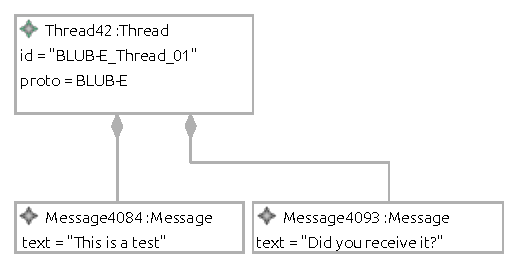
\includegraphics{images/04_transformation_framework/instance_models_combination/chat_instance_partial1.pdf}
        \caption{The chat application instance model $Im_{Chat}$}
        \label{fig:transformation_framework:instance_models_and_instance_graphs:combining_instance_models:combine_example_imod1}
    \end{subfigure}
    \par\medskip
    \begin{subfigure}{\textwidth}
        \centering
        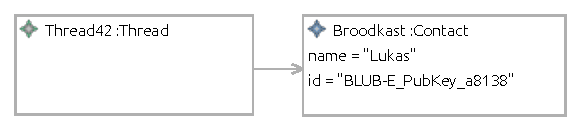
\includegraphics{images/04_transformation_framework/instance_models_combination/chat_instance_partial2.pdf}
        \caption{The contact extension instance model $Im_{Extension}$}
        \label{fig:transformation_framework:instance_models_and_instance_graphs:combining_instance_models:combine_example_imod2}
    \end{subfigure}
    \par\medskip
    \begin{subfigure}{\textwidth}
        \centering
        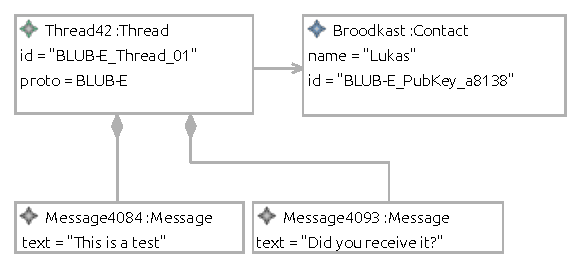
\includegraphics{images/04_transformation_framework/instance_models_combination/chat_instance_combined.pdf}
        \caption{The extended chat application instance model $Im_{ChatExt}$}
        \label{fig:transformation_framework:instance_models_and_instance_graphs:combining_instance_models:combine_example_imod12}
    \end{subfigure}
    \caption{Example of the combination of type models}
    \label{fig:transformation_framework:instance_models_and_instance_graphs:combining_instance_models:combine_example}
\end{figure}

Although the definitions of the combination of instance models are given, no mathematical properties or theorems are defined yet. Some mathematical properties hold for the combination of instance models, that will be presented in the following theorems.

\begin{thm}[Commutativity of the combination of instance models]
\label{defin:transformation_framework:instance_models_and_instance_graphs:combining_instance_models:imod_combine_commute}
Assume that $Im_A$ and $Im_B$ are instance models, then the $\mathrm{combine}$ function is commutative:
\begin{equation*}
    \mathrm{combine}(Im_A, Im_B) = \mathrm{combine}(Im_B, Im_A)
\end{equation*}
\isabellelref{imod_combine_commute}{Ecore.Instance_Model_Combination}
\end{thm}

\begin{thm}[Associativity of the combination of instance models]
\label{defin:transformation_framework:instance_models_and_instance_graphs:combining_instance_models:imod_combine_assoc}
Assume that $Im_A$, $Im_B$ and $Im_C$ are instance models, then the $\mathrm{combine}$ function is associative:
\begin{equation*}
    \mathrm{combine}(\mathrm{combine}(Im_A, Im_B), Im_C) = \mathrm{combine}(Im_A, \mathrm{combine}(Im_B, Im_C))
\end{equation*}
\isabellelref{imod_combine_assoc}{Ecore.Instance_Model_Combination}
\end{thm}

\begin{thm}[Idempotence of the combination of instance models]
\label{defin:transformation_framework:instance_models_and_instance_graphs:combining_instance_models:imod_combine_idemp}
Assume that $Im_A$ is an instance model and that it is valid in the sense of \cref{defin:formalisations:ecore_formalisation:instance_models:model_validity}. Then the following property holds:
\begin{equation*}
    \mathrm{combine}(Im_A, Im_A) = Im_A
\end{equation*}
\isabellelref{imod_combine_idemp_alt}{Ecore.Instance_Model_Combination}
\end{thm}

These properties follow directly from \cref{defin:transformation_framework:instance_models_and_instance_graphs:combining_instance_models:combine}, but the corresponding proofs will not be included here. It should be noted that these properties are indeed proven correct as part of this thesis, and the corresponding proofs are validated within Isabelle.

Besides these properties, the combination of instance models also has an identity element. The empty instance model represents this identity element, but it needs to be defined first:

\begin{defin}[Empty instance model]
\label{defin:transformation_framework:instance_models_and_instance_graphs:combining_instance_models:empty_instance_model}
Let $Im_{\epsilon}$ be the empty instance model. It is typed by the empty type model $Tm_{\epsilon}$. $Im_{\epsilon}$ is defined as:
\begin{align*}
Im_{\epsilon} = \langle&
Object = \{\} \\&
\mathrm{ObjectClass} = undefined \\&
\mathrm{ObjectId} = undefined \\&
\mathrm{FieldValue} = undefined \\&
\mathrm{DefaultValue} = undefined\rangle
\end{align*}
\end{defin}

\begin{thm}[Correctness of the empty type model]
\label{defin:transformation_framework:instance_models_and_instance_graphs:combining_instance_models:imod_empty_correct}
The empty instance model, $Im_{\epsilon}$, is valid with respect to
\cref{defin:formalisations:ecore_formalisation:instance_models:model_validity}.
\isabellelref{imod_empty_correct}{Ecore.Instance_Model}
\end{thm}

The proof for the correctness of the empty instance model is trivial. Still, a validated version of this proof can be found within the Isabelle theories of this thesis.

As mentioned earlier, the empty instance model acts as an identity element when combining two instance models. The following theorem specifies this behaviour.

\begin{thm}[Identity of the combination of instance models]
\label{defin:transformation_framework:instance_models_and_instance_graphs:combining_instance_models:imod_combine_identity}
Assume that $Im_A$ is an instance model and that it is valid in the sense of \cref{defin:formalisations:ecore_formalisation:instance_models:model_validity}. Then $Im_{\epsilon}$ acts as an identity element in the combination function:
\begin{equation*}
    \mathrm{combine}(Im_{\epsilon}, Im_A) = Im_A
\end{equation*}
\isabellelref{imod_combine_identity_alt}{Ecore.Instance_Model_Combination}
\end{thm}

Once more, the proof of this theorem follows directly from the definition. Therefore, the corresponding proof will not be included here, but a validated version can be found within the Isabelle theories of this thesis.

A final desired property for the combination of instance models is a correctness property. \cref{defin:transformation_framework:instance_models_and_instance_graphs:combining_instance_models:imod_combine_correct} defines the theorem under which the combination of instance models is a valid instance model. Please note that this theorem is a generic theorem, which does not take into account that the instance models are mostly distinct.

\begin{thm}[Validity of the combination of instance models]
\label{defin:transformation_framework:instance_models_and_instance_graphs:combining_instance_models:imod_combine_correct}
Assume that $Im_A$ and $Im_B$ are valid instance models in the sense of \cref{defin:formalisations:ecore_formalisation:instance_models:model_validity}. Assume that $Im_A$ is typed by type model $Tm_A$. Furthermore, assume that $Im_B$ is typed by type model $Tm_B$. $Tm_A$ and $Tm_B$ are consistent by definition. Also assume that $Tm_{AB} = \mathrm{combine}(Tm_A, Tm_B)$ is consistent in the sense of \cref{defin:formalisations:ecore_formalisation:type_models:type_model_consistency}. Finally, assume the following properties:
\begin{itemize}
    \item For all shared objects, the object class must be the same in both instance models: $\forall o \in Object_{Im_A} \cap Object_{Im_B}\!: \mathrm{ObjectClass}_{Im_A}(o) = \mathrm{ObjectClass}_{Im_B}(o)$.
    \item For all shared objects, the object id must be the same in both instance models: $\forall o \in Object_{Im_A} \cap Object_{Im_B}\!: \mathrm{ObjectId}_{Im_A}(o) = \mathrm{ObjectId}_{Im_B}(o)$.
    \item For all shared constants within the corresponding type graphs, the default value must be the same in both instance models: $\forall c \in Constant_{Tm_A} \cap Constant_{Tm_B}\!:$\\$\mathrm{DefaultValue}_{Im_A}(c) = \mathrm{DefaultValue}_{Im_B}(c)$.
    \item The identifiers must be unique across both instance models: $\forall o_1 \in Object_{Im_A} \setminus Object_{Im_B} \land o_2 \in Object_{Im_B} \setminus Object_{Im_A}\!: \mathrm{ObjectId}_{Im_A}(o_1) = \mathrm{ObjectId}_{Im_B}(o_2) \implies o_1 = o_2$.
    \item If a field value is set for a combination of an object and field in both instance models, that field value must be the same in both instance models: $\forall o \in Object_{Im_A} \cap Object_{Im_B}\ \land$\\$f \in \mathrm{fields}_{Tm_A}(\mathrm{ObjectClass}_{Im_A}(o)) \cap \mathrm{fields}_{Tm_B}(\mathrm{ObjectClass}_{Im_B}(o))\!:$\\$\mathrm{FieldValue}_{Im_A}(( o, f )) = \mathrm{FieldValue}_{Im_B}(( o, f ))$.
    \item If an object needs a field value in the combination of $Im_A$ and $Im_B$, but this field value is not set in $Im_A$, then it must be set in $Im_B$:
    $\forall o \in Object_{Im_A} \land f \not\in \mathrm{fields}_{Tm_A}(\mathrm{ObjectClass}_{Im_A}(o))\!:
    f \in \mathrm{fields}_{Tm_{AB}}(\mathrm{ObjectClass}_{\mathrm{combine}(Im_A, Im_B)}(o)) \implies$\\$
    o \in Object_{Im_B} \land f \in \mathrm{fields}_{Tm_B}(\mathrm{ObjectClass}_{Im_B}(o))$.
    \item If an object needs a field value in the combination of $Im_A$ and $Im_B$, but this field value is not set in $Im_B$, then it must be set in $Im_A$:
    $\forall o \in Object_{Im_B} \land f \not\in \mathrm{fields}_{Tm_B}(\mathrm{ObjectClass}_{Im_B}(o))\!:
    f \in \mathrm{fields}_{Tm_{AB}}(\mathrm{ObjectClass}_{\mathrm{combine}(Im_A, Im_B)}(o)) \implies$\\$
    o \in Object_{Im_A} \land f \in \mathrm{fields}_{Tm_A}(\mathrm{ObjectClass}_{Im_A}(o))$.
    \item For field values copied from $Im_A$ that are in $ContainerValue_{Im_A}$, the combined multiplicity must be correct: $\forall o \in Object_{Im_A}\ \land f \in \mathrm{fields}_{Tm_A}(\mathrm{ObjectClass}_{Im_A}(o))\ \land$\\$f \in Field_{Tm_B}\!: \mathrm{FieldValue}_{Im_A}(( o, f )) \in ContainerValue_{Im_A} \implies$\\$\mathrm{lower}_{Tm_{AB}}(\mathrm{FieldSig}_{Tm_{AB}}(f)) \leq |\mathrm{FieldValue}_{Im_A}(( o, f ))|\ \land$\\$|\mathrm{FieldValue}_{Im_A}(( o, f ))| \leq \mathrm{upper}_{Tm_{AB}}(\mathrm{FieldSig}_{Tm_{AB}}(f))$.
    \item For field values copied from $Im_B$ that are in $ContainerValue_{Im_B}$, the combined multiplicity must be correct: $\forall o \in Object_{Im_B}\ \land f \in \mathrm{fields}_{Tm_B}(\mathrm{ObjectClass}_{Im_B}(o))\ \land$\\$f \in Field_{Tm_A}\!: \mathrm{FieldValue}_{Im_B}(( o, f )) \in ContainerValue_{Im_B} \implies$\\$\mathrm{lower}_{Tm_{AB}}(\mathrm{FieldSig}_{Tm_{AB}}(f)) \leq |\mathrm{FieldValue}_{Im_B}(( o, f ))|\ \land$\\$|\mathrm{FieldValue}_{Im_B}(( o, f ))| \leq \mathrm{upper}_{Tm_{AB}}(\mathrm{FieldSig}_{Tm_{AB}}(f))$.
    \item If there exists a containment property in $Tm_{AB}$, the satisfaction formula for containment properties must be satisfied: $\forall o \in Object_{Im_A} \cup Object_{Im_B}\!:$\\$\big|\big\{ \big( ( f\!o, f\!\!f ), f\!v \big) \mid \big( ( f\!o, f\!\!f ), fv \big) \in \mathrm{FieldValue}_{\mathrm{combine}(Im_A, Im_B)} \land [ \type{obj}, o ] = f\!v \land f\!\!f \in CR_{Tm_{AB}} \big\}\big| \leq 1$
    \item There may be no cycles in the containment edges of the combined instance model: $\big\{ (f\!o, f\!v) \mid \big( ( f\!o, f\!\!f ), f\!v \big) \in \mathrm{FieldValue}_{\mathrm{combine}(Im_A, Im_B)} \land f\!\!f \in CR_{Tm_{AB}} \big\}$ is acyclic.
    \item The identity properties must remain satisfied when combining objects from different instance models: $\forall [ \type{identity}, c, A ] \in Prop_{Tm_{A}} \land [ \type{identity}, c, A ] \in Prop_{Tm_{B}} \land o_1 \in Object_{Im_A} \setminus Object_{Im_B} \land o_2 \in Object_{Im_B} \setminus Object_{Im_A} \land \mathrm{ObjectClass}_{Im_A}(o_1) = c \land \mathrm{ObjectClass}_{Im_B}(o_2) = c \land a \in A\!: \mathrm{FieldValue}_{Im_A}(( o_1, a )) \equiv_{\mathrm{combine}(Im_A, Im_B)} \mathrm{FieldValue}_{Im_B}(( o_2, a )) \implies o_1 = o_2$.
    \item The opposite properties must remain satisfied when combining objects from different instance models: $\forall [ \type{opposite}, r_1, r_2 ] \in Prop_{Tm_{A}} \land [ \type{opposite}, r_1, r_2 ] \in Prop_{Tm_{B}}\ \land$\\$o_1 \in Object_{Im_A} \land (o_1 \not\in Object_{Im_B} \lor r_1 \not\in \mathrm{fields}_{Tm_B}(\mathrm{ObjectClass}_{Im_B}(o_1)))\ \land$\\$o_2 \in Object_{Im_B} \land (o_2 \not\in Object_{Im_A} \lor r_2 \not\in \mathrm{fields}_{Tm_A}(\mathrm{ObjectClass}_{Im_A}(o_2))) \implies$\\$ \mathrm{edgeCount}_{Im_A}(o_1, r_1, o_2) = \mathrm{edgeCount}_{Im_B}(o_2, r_2, o_1)$.
\end{itemize}

Then $\mathrm{combine}(Im_A, Im_B)$ is a valid instance model in the sense of \cref{defin:formalisations:ecore_formalisation:instance_models:model_validity}
\isabellelref{imod_combine_correct}{Ecore.Instance_Model_Combination}
\end{thm}

\begin{proof}
To proof that $\mathrm{combine}(Im_A, Im_B)$ is a valid instance model, it needs to be shown that\\ $\mathrm{combine}(Im_A, Im_B)$ gives rise to a valid structure for an instance model and that \cref{defin:formalisations:ecore_formalisation:instance_models:model_validity} holds. For readability, define $Im_{AB}$ to be $\mathrm{combine}(Im_A, Im_B)$.

\emph{Structural properties}
\begin{itemize}
    \item For each object $o$, $\mathrm{ObjectClass}_{Im_{AB}}(o)$ must be an element of $Class_{Tm_{AB}}$.

    If $o \in Object_{Im_A} \setminus Object_{Im_B}$, then $\mathrm{ObjectClass}_{Im_{AB}}(o) \in Class_{Tm_{AB}}$.
    
    Similarly, if $o \in Object_{Im_B} \setminus Object_{Im_A}$, then $\mathrm{ObjectClass}_{Im_{AB}}(o) \in Class_{Tm_{AB}}$.
    
    If $o \in Object_{Im_A} \cap Object_{Im_B}$, then $\mathrm{ObjectClass}_{Im_{A}}(o) = \mathrm{ObjectClass}_{Im_{B}}(o)$ by assumption. Therefore $\mathrm{ObjectClass}_{Im_{AB}}(o) \in Class_{Tm_{AB}}$.


    \item For each object $o$, $\mathrm{ObjectId}_{Im_{AB}}(o)$ must be an element of $Name$.
    
    If $o \in Object_{Im_A} \setminus Object_{Im_B}$, then $\mathrm{ObjectId}_{Im_{AB}}(o) \in Name$.
    
    Similarly, if $o \in Object_{Im_B} \setminus Object_{Im_A}$, then $\mathrm{ObjectId}_{Im_{AB}}(o) \in Name$.
    
    If $o \in Object_{Im_A} \cap Object_{Im_B}$, then $\mathrm{ObjectId}_{Im_{A}}(o) = \mathrm{ObjectId}_{Im_{B}}(o)$ by assumption. Therefore $\mathrm{ObjectId}_{Im_{AB}}(o) \in Name$.
    
    
    \item For each object $o$, and $f \in \mathrm{fields}_{Tm_{AB}}(\mathrm{ObjectClass}_{Im_{AB}}(o))$, $\mathrm{FieldValue}_{Im_{AB}}(( o, f ))$ must be an element of $Value_{Im_{AB}}$.
    
    First, note that $Value_{Im_A} \cup Value_{Im_B} \subseteq Value_{Im_{AB}}$\\(see \isabelleref{imod_combine_value}{Ecore.Instance_Model_Combination}).
    
    If $o \in Object_{Im_A} \setminus Object_{Im_B}$, then $f \in \mathrm{fields}_{Tm_{A}}(\mathrm{ObjectClass}_{Im_{A}}(o))$ or \\$f \not\in \mathrm{fields}_{Tm_{A}}(\mathrm{ObjectClass}_{Im_{A}}(o))$.
    
    \begin{itemize}
        \item If $f \in \mathrm{fields}_{Tm_{A}}(\mathrm{ObjectClass}_{Im_{A}}(o))$, then $\mathrm{FieldValue}_{Im_{AB}}(( o, f )) = \mathrm{FieldValue}_{Im_{A}}(( o, f ))$ and, therefore, $\mathrm{FieldValue}_{Im_{AB}}(( o, f )) \in Value_{Im_{AB}}$.
        
        \item If $f \not\in \mathrm{fields}_{Tm_{A}}(\mathrm{ObjectClass}_{Im_{A}}(o))$, then by assumption, $f \in Object_{Im_B}$. However, $f \not\in Object_{Im_B}$, so this case is invalid.
    \end{itemize}
    
    If $o \in Object_{Im_B} \setminus Object_{Im_A}$, then $f \in \mathrm{fields}_{Tm_{B}}(\mathrm{ObjectClass}_{Im_{B}}(o))$ or \\$f \not\in \mathrm{fields}_{Tm_{B}}(\mathrm{ObjectClass}_{Im_{B}}(o))$.
    
    \begin{itemize}
        \item If $f \in \mathrm{fields}_{Tm_{B}}(\mathrm{ObjectClass}_{Im_{B}}(o))$, then $\mathrm{FieldValue}_{Im_{AB}}(( o, f )) = \mathrm{FieldValue}_{Im_{B}}(( o, f ))$ and, therefore, $\mathrm{FieldValue}_{Im_{AB}}(( o, f )) \in Value_{Im_{AB}}$.
        
        \item If $f \not\in \mathrm{fields}_{Tm_{B}}(\mathrm{ObjectClass}_{Im_{B}}(o))$, then by assumption, $f \in Object_{Im_A}$. However, $f \not\in Object_{Im_A}$, so this case is invalid.
    \end{itemize}
    
    If $o \in Object_{Im_A} \cap Object_{Im_B}$, then \\$f \in \mathrm{fields}_{Tm_{A}}(\mathrm{ObjectClass}_{Im_{A}}(o)) \cap \mathrm{fields}_{Tm_{B}}(\mathrm{ObjectClass}_{Im_{B}}(o))$ or \\$f \not\in \mathrm{fields}_{Tm_{A}}(\mathrm{ObjectClass}_{Im_{A}}(o))$ or $f \not\in \mathrm{fields}_{Tm_{B}}(\mathrm{ObjectClass}_{Im_{B}}(o))$.
    
    \begin{itemize}
        \item If $f \in \mathrm{fields}_{Tm_{A}}(\mathrm{ObjectClass}_{Im_{A}}(o)) \cap \mathrm{fields}_{Tm_{B}}(\mathrm{ObjectClass}_{Im_{B}}(o))$, then \\$\mathrm{FieldValue}_{Im_{AB}}(( o, f )) = \mathrm{FieldValue}_{Im_{A}}(( o, f ))$ and, therefore, \\$\mathrm{FieldValue}_{Im_{AB}}(( o, f )) \in Value_{Im_{AB}}$.
        
        \item If $f \not\in \mathrm{fields}_{Tm_{A}}(\mathrm{ObjectClass}_{Im_{A}}(o))$, then by assumption, $f \in \mathrm{fields}_{Tm_{B}}(\mathrm{ObjectClass}_{Im_{B}}(o))$. Therefore, $\mathrm{FieldValue}_{Im_{AB}}(( o, f )) = \mathrm{FieldValue}_{Im_{B}}(( o, f ))$ which means that \\$\mathrm{FieldValue}_{Im_{AB}}(( o, f )) \in Value_{Im_{AB}}$.
        
        \item If $f \not\in \mathrm{fields}_{Tm_{B}}(\mathrm{ObjectClass}_{Im_{B}}(o))$, then by assumption, $f \in \mathrm{fields}_{Tm_{A}}(\mathrm{ObjectClass}_{Im_{A}}(o))$. Therefore, $\mathrm{FieldValue}_{Im_{AB}}(( o, f )) = \mathrm{FieldValue}_{Im_{A}}(( o, f ))$ which means that \\$\mathrm{FieldValue}_{Im_{AB}}(( o, f )) \in Value_{Im_{AB}}$.
    \end{itemize}
    
    
    \item For each constant $c$ in $Constant_{Tm_{AB}}$, $\mathrm{DefaultValue}_{Im_{AB}}(c)$ must be an element of $Value_{Im_{AB}}$.
    
    First, note that $Value_{Im_A} \cup Value_{Im_B} \subseteq Value_{Im_{AB}}$\\(see \isabelleref{imod_combine_value}{Ecore.Instance_Model_Combination}).
    
    If $c \in Constant_{Tm_A} \setminus Constant_{Tm_B}$, then $\mathrm{DefaultValue}_{Im_{AB}}(c) \in Value_{Im_{AB}}$.
    
    Similarly, if $c \in Constant_{Tm_B} \setminus Constant_{Tm_A}$, then $\mathrm{DefaultValue}_{Im_{AB}}(c) \in Value_{Im_{AB}}$.
    
    If $c \in Constant_{Tm_A} \cap Constant_{Tm_B}$, then $\mathrm{DefaultValue}_{Im_{A}}(c) = \mathrm{DefaultValue}_{Im_{B}}(c)$ by assumption. Therefore $\mathrm{DefaultValue}_{Im_{AB}}(c) \in Value_{Im_{AB}}$.
\end{itemize}

\emph{Validity properties}
\begin{itemize}
    \item $\forall (( o, f ), v ) \in \mathrm{FieldValue}_{Im_{AB}}\!: v:_{Im} \mathrm{type}_{Tm_{AB}}(f)$
    
    If $o \in Object_{Im_A} \setminus Object_{Im_B}$, then $f \in \mathrm{fields}_{Tm_{A}}(\mathrm{ObjectClass}_{Im_{A}}(o))$ or \\$f \not\in \mathrm{fields}_{Tm_{A}}(\mathrm{ObjectClass}_{Im_{A}}(o))$.
    
    \begin{itemize}
        \item If $f \in \mathrm{fields}_{Tm_{A}}(\mathrm{ObjectClass}_{Im_{A}}(o))$, then $\mathrm{FieldValue}_{Im_{AB}}(( o, f )) = \mathrm{FieldValue}_{Im_{A}}(( o, f ))$. In this case $\mathrm{type}_{Tm_{AB}}(f) = \mathrm{type}_{Tm_{A}}(f)$ because types are preserved by $Tm_{AB}$. Therefore, $v:_{Im} \mathrm{type}_{Tm_{AB}}(f)$.
        
        \item If $f \not\in \mathrm{fields}_{Tm_{A}}(\mathrm{ObjectClass}_{Im_{A}}(o))$, then by assumption, $f \in Object_{Im_B}$. However, $f \not\in Object_{Im_B}$, so this case is invalid.
    \end{itemize}
    
    If $o \in Object_{Im_B} \setminus Object_{Im_A}$, then $f \in \mathrm{fields}_{Tm_{B}}(\mathrm{ObjectClass}_{Im_{B}}(o))$ or \\$f \not\in \mathrm{fields}_{Tm_{B}}(\mathrm{ObjectClass}_{Im_{B}}(o))$.
    
    \begin{itemize}
        \item If $f \in \mathrm{fields}_{Tm_{B}}(\mathrm{ObjectClass}_{Im_{B}}(o))$, then $\mathrm{FieldValue}_{Im_{AB}}(( o, f )) = \mathrm{FieldValue}_{Im_{B}}(( o, f ))$. In this case $\mathrm{type}_{Tm_{AB}}(f) = \mathrm{type}_{Tm_{B}}(f)$ because types are preserved by $Tm_{AB}$. Therefore, $v:_{Im} \mathrm{type}_{Tm_{AB}}(f)$.
        
        \item If $f \not\in \mathrm{fields}_{Tm_{B}}(\mathrm{ObjectClass}_{Im_{B}}(o))$, then by assumption, $f \in Object_{Im_A}$. However, $f \not\in Object_{Im_A}$, so this case is invalid.
    \end{itemize}
    
    If $o \in Object_{Im_A} \cap Object_{Im_B}$, then \\$f \in \mathrm{fields}_{Tm_{A}}(\mathrm{ObjectClass}_{Im_{A}}(o)) \cap \mathrm{fields}_{Tm_{B}}(\mathrm{ObjectClass}_{Im_{B}}(o))$ or \\$f \not\in \mathrm{fields}_{Tm_{A}}(\mathrm{ObjectClass}_{Im_{A}}(o))$ or $f \not\in \mathrm{fields}_{Tm_{B}}(\mathrm{ObjectClass}_{Im_{B}}(o))$.
    
    \begin{itemize}
        \item If $f \in \mathrm{fields}_{Tm_{A}}(\mathrm{ObjectClass}_{Im_{A}}(o)) \cap \mathrm{fields}_{Tm_{B}}(\mathrm{ObjectClass}_{Im_{B}}(o))$, then \\$\mathrm{FieldValue}_{Im_{AB}}(( o, f )) = \mathrm{FieldValue}_{Im_{A}}(( o, f ))$. In this case $\mathrm{type}_{Tm_{AB}}(f) = \mathrm{type}_{Tm_{A}}(f)$ because types are preserved by $Tm_{AB}$. Therefore, $v:_{Im} \mathrm{type}_{Tm_{AB}}(f)$.
        
        \item If $f \not\in \mathrm{fields}_{Tm_{A}}(\mathrm{ObjectClass}_{Im_{A}}(o))$, then by assumption, $f \in \mathrm{fields}_{Tm_{B}}(\mathrm{ObjectClass}_{Im_{B}}(o))$. Therefore, $\mathrm{FieldValue}_{Im_{AB}}(( o, f )) = \mathrm{FieldValue}_{Im_{B}}(( o, f ))$. Furthermore, $\mathrm{type}_{Tm_{AB}}(f) = \mathrm{type}_{Tm_{A}}(f)$ because types are preserved by $Tm_{AB}$. Therefore, $v:_{Im} \mathrm{type}_{Tm_{AB}}(f)$.
        
        \item If $f \not\in \mathrm{fields}_{Tm_{B}}(\mathrm{ObjectClass}_{Im_{B}}(o))$, then by assumption, $f \in \mathrm{fields}_{Tm_{A}}(\mathrm{ObjectClass}_{Im_{A}}(o))$. Therefore, $\mathrm{FieldValue}_{Im_{AB}}(( o, f )) = \mathrm{FieldValue}_{Im_{A}}(( o, f ))$. Furthermore, $\mathrm{type}_{Tm_{AB}}(f) = \mathrm{type}_{Tm_{A}}(f)$ because types are preserved by $Tm_{AB}$. Therefore, $v:_{Im} \mathrm{type}_{Tm_{AB}}(f)$.
    \end{itemize}
    
    
    \item $\forall (( o, f ), v ) \in \mathrm{FieldValue}_{Im_{AB}}\!: \mathrm{validMul}_{Im_{AB}}(v)$.
    
    If $o \in Object_{Im_A} \setminus Object_{Im_B}$, then $f \in \mathrm{fields}_{Tm_{A}}(\mathrm{ObjectClass}_{Im_{A}}(o))$ or \\$f \not\in \mathrm{fields}_{Tm_{A}}(\mathrm{ObjectClass}_{Im_{A}}(o))$.
    
    \begin{itemize}
        \item If $f \in \mathrm{fields}_{Tm_{A}}(\mathrm{ObjectClass}_{Im_{A}}(o))$, then $\mathrm{FieldValue}_{Im_{AB}}(( o, f )) = \mathrm{FieldValue}_{Im_{A}}(( o, f ))$. Because $Im_{A}$ is valid, $\mathrm{validMul}_{Im_{A}}(v)$ holds. If the multiplicity is preserved because $f \not\in Field_{Tm_B}$, then $\mathrm{validMul}_{Im_{AB}}(v)$. If the multiplicity is changed because $f \in Field_{Tm_B}$, then $\mathrm{validMul}_{Im_{AB}}(v)$ is proven by assumption.
        
        \item If $f \not\in \mathrm{fields}_{Tm_{A}}(\mathrm{ObjectClass}_{Im_{A}}(o))$, then by assumption, $f \in Object_{Im_B}$. However, $f \not\in Object_{Im_B}$, so this case is invalid.
    \end{itemize}
    
    If $o \in Object_{Im_B} \setminus Object_{Im_A}$, then $f \in \mathrm{fields}_{Tm_{B}}(\mathrm{ObjectClass}_{Im_{B}}(o))$ or \\$f \not\in \mathrm{fields}_{Tm_{B}}(\mathrm{ObjectClass}_{Im_{B}}(o))$.
    
    \begin{itemize}
        \item If $f \in \mathrm{fields}_{Tm_{B}}(\mathrm{ObjectClass}_{Im_{B}}(o))$, then $\mathrm{FieldValue}_{Im_{AB}}(( o, f )) = \mathrm{FieldValue}_{Im_{B}}(( o, f ))$. Because $Im_{B}$ is valid, $\mathrm{validMul}_{Im_{B}}(v)$ holds. If the multiplicity is preserved because $f \not\in Field_{Tm_A}$, then $\mathrm{validMul}_{Im_{AB}}(v)$. If the multiplicity is changed because $f \in Field_{Tm_A}$, then $\mathrm{validMul}_{Im_{AB}}(v)$ is proven by assumption.
        
        \item If $f \not\in \mathrm{fields}_{Tm_{B}}(\mathrm{ObjectClass}_{Im_{B}}(o))$, then by assumption, $f \in Object_{Im_A}$. However, $f \not\in Object_{Im_A}$, so this case is invalid.
    \end{itemize}
    
    If $o \in Object_{Im_A} \cap Object_{Im_B}$, then \\$f \in \mathrm{fields}_{Tm_{A}}(\mathrm{ObjectClass}_{Im_{A}}(o)) \cap \mathrm{fields}_{Tm_{B}}(\mathrm{ObjectClass}_{Im_{B}}(o))$ or \\$f \not\in \mathrm{fields}_{Tm_{A}}(\mathrm{ObjectClass}_{Im_{A}}(o))$ or $f \not\in \mathrm{fields}_{Tm_{B}}(\mathrm{ObjectClass}_{Im_{B}}(o))$.
    
    \begin{itemize}
        \item If $f \in \mathrm{fields}_{Tm_{A}}(\mathrm{ObjectClass}_{Im_{A}}(o)) \cap \mathrm{fields}_{Tm_{B}}(\mathrm{ObjectClass}_{Im_{B}}(o))$, then \\$\mathrm{FieldValue}_{Im_{AB}}(( o, f )) = \mathrm{FieldValue}_{Im_{A}}(( o, f ))$. In this case $\mathrm{validMul}_{Im_{AB}}(v)$ is proven by assumption since the multiplicity of $f$ has been combined into a new multiplicity.
        
        \item If $f \not\in \mathrm{fields}_{Tm_{A}}(\mathrm{ObjectClass}_{Im_{A}}(o))$, then by assumption, $f \in \mathrm{fields}_{Tm_{B}}(\mathrm{ObjectClass}_{Im_{B}}(o))$. Therefore, $\mathrm{FieldValue}_{Im_{AB}}(( o, f )) = \mathrm{FieldValue}_{Im_{B}}(( o, f ))$. Furthermore, because $Im_{B}$ is valid, $\mathrm{validMul}_{Im_{B}}(v)$ holds. If the multiplicity is preserved because $f \not\in Field_{Tm_A}$, then $\mathrm{validMul}_{Im_{AB}}(v)$. If the multiplicity is changed because $f \in Field_{Tm_A}$, then $\mathrm{validMul}_{Im_{AB}}(v)$ is proven by assumption.
        
        \item If $f \not\in \mathrm{fields}_{Tm_{B}}(\mathrm{ObjectClass}_{Im_{B}}(o))$, then by assumption, $f \in \mathrm{fields}_{Tm_{A}}(\mathrm{ObjectClass}_{Im_{A}}(o))$. Therefore, $\mathrm{FieldValue}_{Im_{AB}}(( o, f )) = \mathrm{FieldValue}_{Im_{A}}(( o, f ))$. Furthermore, because $Im_{A}$ is valid, $\mathrm{validMul}_{Im_{A}}(v)$ holds. If the multiplicity is preserved because $f \not\in Field_{Tm_B}$, then $\mathrm{validMul}_{Im_{AB}}(v)$. If the multiplicity is changed because $f \in Field_{Tm_B}$, then $\mathrm{validMul}_{Im_{AB}}(v)$ is proven by assumption.
    \end{itemize}
    
    
    \item $\forall p \in Prop_{Tm_{AB}}\!: Im \models p$
    
    Make a case distinction for the different possible properties.
    \begin{itemize}
        \item For $[ \type{abstract}, c ] \in Prop_{Tm_{AB}}$, use the fact that $Tm_{AB}$ is consistent to establish that abstract properties are only copied iff there are no instances of it in the combined instance graph (see \cref{defin:transformation_framework:type_models_and_type_graphs:combining_type_models:prop_combine} for details). Therefore, $Im \models [ \type{abstract}, c ]$.
        
        \item For $[ \type{containment}, r ] \in Prop_{Tm_{AB}}$, use the assumptions to prove that $Im \models [ \type{containment}, r ]$.
        
        \item For $[ \type{defaultValue}, f, v ] \in Prop_{Tm_{AB}}$, there is no specific satisfaction formula, therefore $Im \models [ \type{defaultValue}, f, v ]$.
        
        \item For $[ \type{identity}, c, A ] \in Prop_{Tm_{AB}}$, if the property was copied over from only one of the type models, then $Im \models [ \type{identity}, c, A ]$. This is the case because $c$ could not have been part of the other type model and therefore not occur in its instance models.
        
        If $[ \type{identity}, c, A ] \in Prop_{Tm_{AB}}$ was present in both type models, then the identity satisfaction formula will be correct for each pair of instances from $Im_{A}$ and each pair of instances from $Im_{B}$. To ensure that it is correct for mixed instance pairs, use the assumption specified. Then establish that $Im \models [ \type{identity}, c, A ]$.
        
        \item For $[ \type{keyset}, r, A ] \in Prop_{Tm_{AB}}$, it is clear that each value of $r$ in the combined instance graph is either the copied field value from $Im_{A}$ or the copied field value from $Im_{B}$. Since values are preserved, there can be no new objects added to an existing relation. Therefore, $Im \models [ \type{keyset}, r, A ]$.
        
        \item For $[ \type{opposite}, r, r' ] \in Prop_{Tm_{AB}}$, if the property was copied over from only one of the type models, then $Im \models [ \type{opposite}, r, r' ]$. This is the case because $r$ and $r'$ could not have been part of the other type model and therefore not occur in its instance models.
        
        If $[ \type{opposite}, r, r' ] \in Prop_{Tm_{AB}}$ was present in both type models, then the opposite satisfaction formula will be correct for each pair of instances from $Im_{A}$ and each pair of instances from $Im_{B}$. To ensure that it is correct for mixed instance pairs, use the assumption specified. Then establish that $Im \models [ \type{opposite}, r, r' ]$.
        
        \item For $[ \type{readonly}, f ] \in Prop_{Tm_{AB}}$, there is no specific satisfaction formula, therefore $Im \models [ \type{readonly}, f ]$.
    \end{itemize}
    
    
    \item $\forall c \in Constant_{Tm_{AB}}\!: \mathrm{DefaultValue}_{Im_{AB}}(c):_{Im_{AB}} \mathrm{ConstType}_{Tm_{AB}}(c)$.
    
    If $c \in Constant_{Tm_A} \setminus Constant_{Tm_B}$, then $\mathrm{DefaultValue}_{Im_{AB}}(c) = \mathrm{DefaultValue}_{Im_{A}}(c)$. Furthermore, $\mathrm{ConstType}_{Tm_{AB}}(c) = \mathrm{ConstType}_{Tm_{A}}(c)$. Therefore, \\$\mathrm{DefaultValue}_{Im_{AB}}(c):_{Im_{AB}} \mathrm{ConstType}_{Tm_{AB}}(c)$.
    
    Similarly, if $c \in Constant_{Tm_B} \setminus Constant_{Tm_A}$, then $\mathrm{DefaultValue}_{Im_{AB}}(c) = \mathrm{DefaultValue}_{Im_{B}}(c)$. Furthermore, $\mathrm{ConstType}_{Tm_{AB}}(c) = \mathrm{ConstType}_{Tm_{B}}(c)$. Therefore, \\$\mathrm{DefaultValue}_{Im_{AB}}(c):_{Im_{AB}} \mathrm{ConstType}_{Tm_{AB}}(c)$.
    
    If $c \in Constant_{Tm_A} \cap Constant_{Tm_B}$, then $\mathrm{DefaultValue}_{Im_{A}}(c) = \mathrm{DefaultValue}_{Im_{B}}(c)$ by assumption. Furthermore, $\mathrm{ConstType}_{Tm_{A}}(c) = \mathrm{ConstType}_{Tm_{B}}(c)$, since $Tm_{AB}$ is consistent. Therefore, $\mathrm{DefaultValue}_{Im_{AB}}(c):_{Im_{AB}} \mathrm{ConstType}_{Tm_{AB}}(c)$.
    
    
    \item $Tm_{AB}$ is consistent, as defined in \cref{defin:formalisations:ecore_formalisation:type_models:type_model_consistency}.
    
    This is specified to be true by assumption.
\end{itemize}

The proofs of all these individual properties complete the entire proof.
\end{proof}

As explained before, \cref{defin:transformation_framework:instance_models_and_instance_graphs:combining_instance_models:imod_combine_correct} does not take into account that the instance models are supposed to be distinct except for a set of objects. Furthermore, it does not take into account that the corresponding type models are supposed to be distinct except for a set of types. The following lemma is an alternation of the previous theorem, which takes these properties into account.

\begin{lem}[Consistency of the combination (mostly) distinct of instance models]
\label{defin:transformation_framework:instance_models_and_instance_graphs:combining_instance_models:imod_combine_merge_correct}
Assume that $Im_A$ and $Im_B$ are valid instance models in the sense of \cref{defin:formalisations:ecore_formalisation:instance_models:model_validity}. Assume that $Im_A$ is typed by type model $Tm_A$. Furthermore, assume that $Im_B$ is typed by type model $Tm_B$. $Tm_A$ and $Tm_B$ are consistent by definition. Also assume that $Tm_{AB} = \mathrm{combine}(Tm_A, Tm_B)$ is consistent in the sense of \cref{defin:formalisations:ecore_formalisation:type_models:type_model_consistency}. Moreover, assume that $Tm_{A}$ and $Tm_{B}$ are entirely distinct except for a set of types $T$. Also assume that $Im_{A}$ and $Im_{B}$ are entirely distinct except for a set of objects $O$. Finally, assume the following properties:
\begin{itemize}
    \item For all shared objects, the object class must be the same in both instance models: $\forall o \in Object_{Im_A} \cap Object_{Im_B}\!: \mathrm{ObjectClass}_{Im_A}(o) = \mathrm{ObjectClass}_{Im_B}(o)$.
    \item For all shared objects, the object id must be the same in both instance models: $\forall o \in Object_{Im_A} \cap Object_{Im_B}\!: \mathrm{ObjectId}_{Im_A}(o) = \mathrm{ObjectId}_{Im_B}(o)$.
    \item For all shared constants within the corresponding type graphs, the default value must be the same in both instance models: $\forall c \in Constant_{Tm_A} \cap Constant_{Tm_B}\!:$\\$\mathrm{DefaultValue}_{Im_A}(c) = \mathrm{DefaultValue}_{Im_B}(c)$.
    \item The identifiers must be unique across both instance models: $\forall o_1 \in Object_{Im_A} \setminus Object_{Im_B} \land o_2 \in Object_{Im_B} \setminus Object_{Im_A}\!: \mathrm{ObjectId}_{Im_A}(o_1) = \mathrm{ObjectId}_{Im_B}(o_2) \implies o_1 = o_2$.
    \item If an object needs a field value in the combination of $Im_A$ and $Im_B$, but this field value is not set in $Im_A$, then it must be set in $Im_B$:
    $\forall o \in Object_{Im_A} \land f \not\in \mathrm{fields}_{Tm_A}(\mathrm{ObjectClass}_{Im_A}(o))\!:
    f \in \mathrm{fields}_{Tm_{AB}}(\mathrm{ObjectClass}_{\mathrm{combine}(Im_A, Im_B)}(o)) \implies$\\$
    o \in Object_{Im_B} \land f \in \mathrm{fields}_{Tm_B}(\mathrm{ObjectClass}_{Im_B}(o))$.
    \item If an object needs a field value in the combination of $Im_A$ and $Im_B$, but this field value is not set in $Im_B$, then it must be set in $Im_A$:
    $\forall o \in Object_{Im_B} \land f \not\in \mathrm{fields}_{Tm_B}(\mathrm{ObjectClass}_{Im_B}(o))\!:
    f \in \mathrm{fields}_{Tm_{AB}}(\mathrm{ObjectClass}_{\mathrm{combine}(Im_A, Im_B)}(o)) \implies$\\$
    o \in Object_{Im_A} \land f \in \mathrm{fields}_{Tm_A}(\mathrm{ObjectClass}_{Im_A}(o))$.
    \item If there exists a containment property in $Tm_{AB}$, the satisfaction formula for containment properties must be satisfied: $\forall o \in Object_{Im_A} \cup Object_{Im_B}\!:$\\$\big|\big\{ \big( ( f\!o, f\!\!f ), f\!v \big) \mid \big( ( f\!o, f\!\!f ), fv \big) \in \mathrm{FieldValue}_{\mathrm{combine}(Im_A, Im_B)} \land [ \type{obj}, o ] = f\!v \land f\!\!f \in CR_{Tm_{AB}} \big\}\big| \leq 1$
    \item There may be no cycles in the containment edges of the combined instance model: $\big\{ (f\!o, f\!v) \mid \big( ( f\!o, f\!\!f ), f\!v \big) \in \mathrm{FieldValue}_{\mathrm{combine}(Im_A, Im_B)} \land f\!\!f \in CR_{Tm_{AB}} \big\}$ is acyclic.
\end{itemize}

Then $\mathrm{combine}(Im_A, Im_B)$ is a valid instance model in the sense of \cref{defin:formalisations:ecore_formalisation:instance_models:model_validity}.
\isabellelref{imod_combine_merge_correct}{Ecore.Instance_Model_Combination}
\end{lem}

\begin{proof}
Use \cref{defin:transformation_framework:instance_models_and_instance_graphs:combining_instance_models:imod_combine_correct} to show that $\mathrm{combine}(Im_A, Im_B)$ is a consistent type model. Use the assumptions given. Some assumptions of \cref{defin:transformation_framework:instance_models_and_instance_graphs:combining_instance_models:imod_combine_correct} become irrelevant because $Im_A$ and $Im_B$ are mostly distinct.
\end{proof}

Finally, the concept of compatibility between two instance models is defined.

\begin{defin}[Compatibility of instance models]
\label{defin:transformation_framework:instance_models_and_instance_graphs:combining_instance_models:compatibility}
Assume instance models $Im_A$ and $Im_B$. We say that $Im_A$ is compatible with $Im_B$ if  $\mathrm{combine}(Im_A, Im_B)$ is a valid instance model in the sense of \cref{defin:formalisations:ecore_formalisation:instance_models:model_validity}.
\end{defin}

The notion of compatibility will be used later as a way to denote instance models that can be combined with other instance models without loss of validity.